% listing style
\definecolor{codegreen}{rgb}{0,0.6,0}
\definecolor{codegray}{rgb}{0.5,0.5,0.5}
\definecolor{codepurple}{rgb}{0.58,0,0.82}
\definecolor{backcolour}{rgb}{0.95,0.95,0.92}

\lstdefinestyle{mystyle}{
    backgroundcolor=\color{backcolour},   
    commentstyle=\color{codegreen},
    keywordstyle=\color{magenta},
    numberstyle=\tiny\color{codegray},
    stringstyle=\color{codepurple},
    basicstyle=\ttfamily\footnotesize,
    breakatwhitespace=false,         
    breaklines=true,                 
    captionpos=b,                    
    keepspaces=true,                 
    numbers=left,                    
    numbersep=5pt,                  
    showspaces=false,                
    showstringspaces=false,
    showtabs=false,                  
    tabsize=2
}

\lstset{style=mystyle}

Ce chapitre décrit les différents services qui composent la pipeline de génération de pochette d'album (cf. \ref{fig:flowchart}).
Ces derniers ont tous été développés en Python et suivent les spécifications du Core Engine du CSIA-PME \cite{CSIA-PME}.

\section{YouTube Downloader}
Le premier service est un service optionnel. En effet, ce dernier s'est ajouté en cours de route pour faciliter l'utilisation de notre application.
Avoir un fichier audio sous la main n'est pas toujours évident, nn downloader YouTube est donc inclus. Ainsi, à l'aide de l'URL d'une vidéo, il est possible de récupérer le son de cette dernière et de l'exploiter.

La librairie utilisée pour ce service s'appelle PyTube. Elle s'occupe de lister les différents flux retournés par l'URL de YouTube et il est ensuite possible de les enregistrer dans le format souhaité. 

Grâce à ce service, on peut donc choisir d'utiliser son propre fichier audio ou d'avoir une étape supplémentaire afin de le récupérer d'Internet.

\section{Speech to Text}

Retrouver les paroles d'un audio est une étape importante dans le processus de génération de pochettes d'album. En effet, afin de pouvoir donner une meilleure instruction au service de génération d'image, il est important de comprendre de quoi parle la musique, ainsi que les sentiments qui y sont liés. 

Après avoir fait un tour des technologies existantes (le but n'étant pas de créer un modèle de zéro), Whisper \cite{openai_whisper} s'est imposé comme étant le plus performant (l'état de l'art). C'est donc ce modèle qui est utilisé, dans sa version 2, pour le service de reconnaissance de parole. Son installation et son utilisation sont très simples, ce qui a permis, assez rapidement, de rendre ce service opérationnel.

À noter qu'il était initialement prévu d'ajouter un service à la pipeline, comme l'illustre la figure \ref{fig:voice_extraction}, qui isole la voix du reste de la musique pour booster les performances de la reconnaissance de paroles. Cette idée à été abandonnée au vu des résultats satisfaisants obtenus avec Whisper.

\begin{figure}[H]
    \begin{center}
        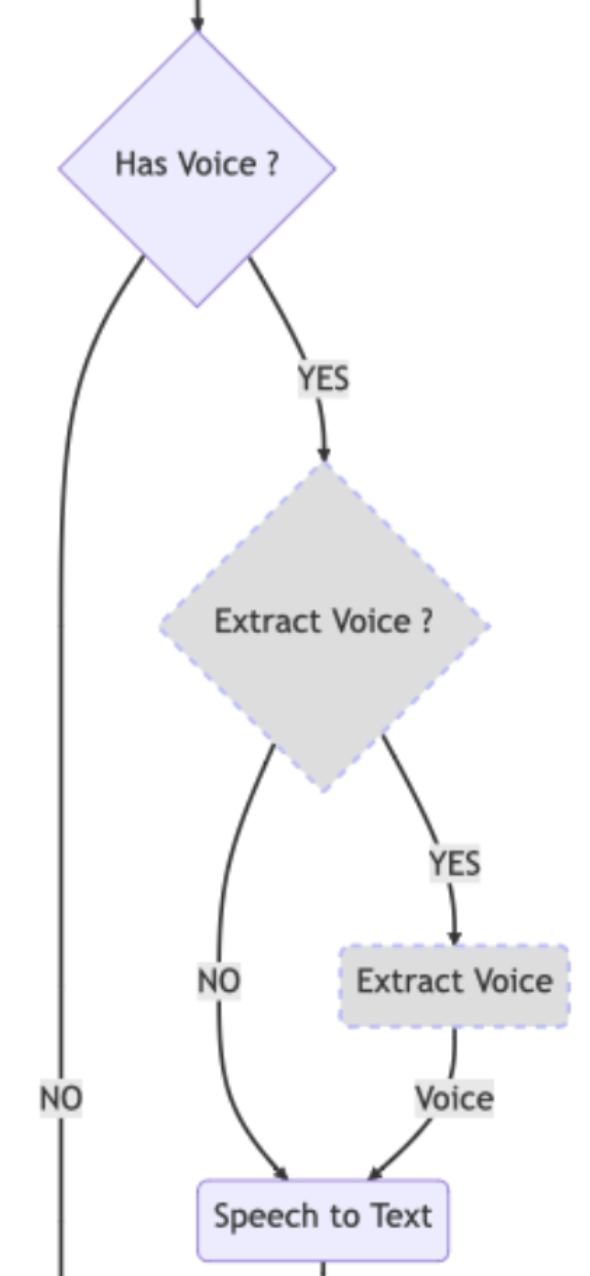
\includegraphics[width=0.25\textwidth]{rapport_PI/rsc/voice_extract.png}
        \caption{Extrait de la pipeline présentée dans le cahier des charges \cite{CDC}}
        \label{fig:voice_extraction}
    \end{center}
\end{figure}

\section{Genre Detection}\label{sec:genre_detection}

Tout comme le service de reconnaissance de la parole, le service de détection de genre musicale prend en entrée directement le fichier audio fournit par l'utilisateur. La détection du genre musical permet d'adapter les images générées à la fin de notre pipeline afin qu'elles correspondent aux codes visuels du genre musical de la musique analysée.

Ce service encapsule un modèle de machine-learning entraîné à partir de zéro, dont la tâche est de classifier une donnée audio vers le genre musical qu'elle représente. Cette section décrit donc les données utilisées pour son entraînement, l'architecture du modèle ainsi que son entraînement et les résultats obtenus.

\subsection{Données utilisées}

Le jeu de données GTZAN \cite{gtzan} est certainement le jeu de données le plus utilisé pour la classification de genre musical. Il contient 1000 fichiers audio de 30 secondes chacun, répartis de manière équilibrée dans 10 genres musicaux différents. Des méta-données sont également fournies pour chaque fichier audio mais ne sont pas utilisées dans ce projet. Étant donné que ce jeu de données est relativement petit, nous utilisons également une partie du jeu de données FMA \cite{fma_dataset} qui contient plus de 100'000 fichiers audio, mais dont les genres musicaux sont très déséquilibrés et ne correspondent pas toujours à ceux présents dans le jeu de données GTZAN. On procède donc à un tri conséquent des données contenues dans ce jeu de données pour ne garder uniquement les fichiers audio dont le genre musical est présent dans le jeu de données GTZAN, excepté pour le genre électronique que nous rajoutons. Nous avons, finalement, 11 genres musicaux différents, leur répartition est illustrée à la figure \ref{fig:genre_distribution}.

\begin{figure}[H]
    \centering
    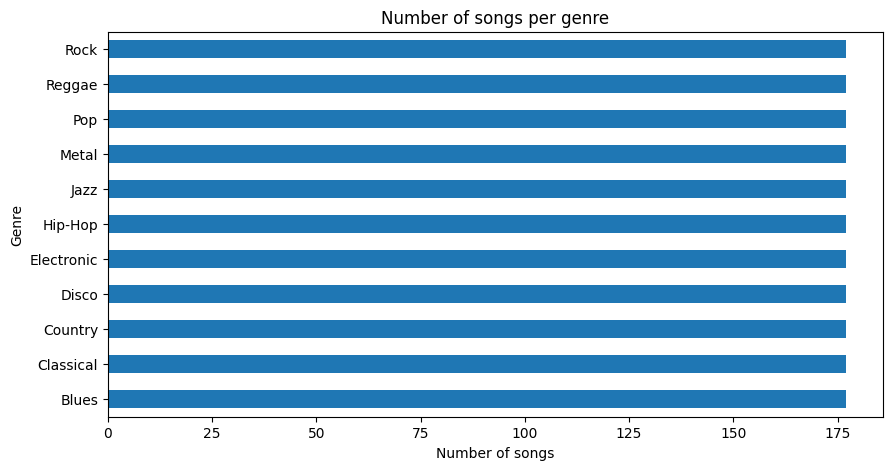
\includegraphics[width=0.8\textwidth]{rsc/genre_distribution.png}
    \caption{Répartition des genres musicaux dans le jeu de données utilisé pour l'entraînement du modèle de détection de genre musical.}
    \label{fig:genre_distribution}
\end{figure}

Nous séparons ensuite le jeu de données en deux parties, une partie pour l'entraînement du modèle (80\%) et une partie pour son évaluation (20\%). Nous obtenons donc 1557 données pour l'entraînement et 390 données pour l'évaluation dont les genres musicaux sont répartis de manière équilibrée.

\subsection{Architecture du modèle}

Plusieurs architectures peuvent être considérées afin de classifier des données audio, les plus utilisées sont les réseaux de neurones récurrents (RNN) et les réseaux de neurones convolutifs (CNN). Dans ce projet, nous utilisons une architecture de CNN créée à la main et inspirée d'un tutoriel en ligne \cite{cnn_tuto}. Les CNN sont particulièrement adaptés à l'analyse d'images mais peuvent également être utilisés pour des données audio. En effet, ces dernières peuvent être représentées sous forme de spectrogrammes, qui sont une représentation graphique de l'évolution de la fréquence d'un signal audio en fonction du temps. Ces spectrogrammes peuvent donc être considérés comme des images et être traités comme telles par un CNN. Dans notre cas, nous générons pour chaque donnée audio un spectrogramme MEL, qui est une variante du spectrogramme classique permettant de capturer plus efficacement les caractéristiques d'un signal audio. La figure \ref{fig:spectrogram} montre un exemple d'un spectrogramme MEL pour chaque canal d'un fichier audio stéréo.

\begin{figure}[H]
    \centering
    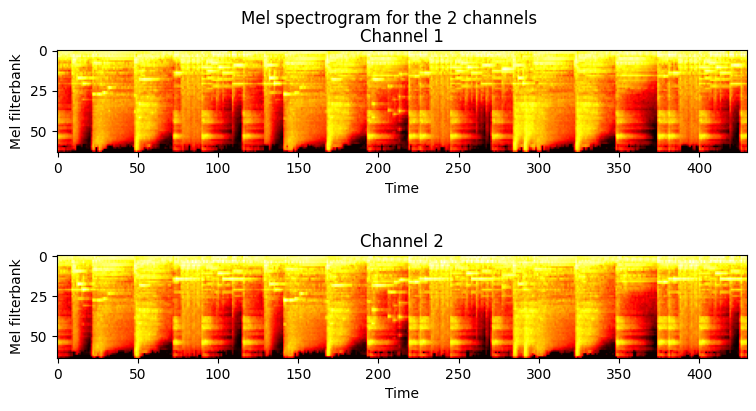
\includegraphics[width=0.6\textwidth]{rsc/spectrogram.png}
    \caption{Spectrogramme MEL pour chaque canal d'un fichier audio stéréo.}
    \label{fig:spectrogram}
\end{figure}

L'architecture du CNN utilisée est globalement assez simple, elle est composée de cinq couches de convolution suivies d'une couche d'\textit{Average Pooling} dont la sortie est directement utilisée pour la classification. Chaque couche de convolution est suivie d'une fonction d'activation ReLU ainsi qu'une couche de \textit{batch normalization} qui permet de stabiliser et d'accélérer l'entraînement du modèle. Le listing \ref{lst:cnn_architecture} décrit l'architecture utilisée.

\begin{lstlisting}[language=Python, caption=Architecture du CNN créé pour notre problème de classification, label=lst:cnn_architecture]
       | Name   | Type              | Params
    ----------------------------------------------
    0  | conv1  | Conv2d            | 408   
    1  | relu1  | ReLU              | 0     
    2  | bn1    | BatchNorm2d       | 16    
    3  | conv2  | Conv2d            | 1.2 K 
    4  | relu2  | ReLU              | 0     
    5  | bn2    | BatchNorm2d       | 32    
    6  | conv3  | Conv2d            | 4.6 K 
    7  | relu3  | ReLU              | 0     
    8  | bn3    | BatchNorm2d       | 64    
    9  | conv4  | Conv2d            | 18.5 K
    10 | relu4  | ReLU              | 0     
    11 | bn4    | BatchNorm2d       | 128   
    12 | conv5  | Conv2d            | 73.9 K
    13 | relu5  | ReLU              | 0     
    14 | bn5    | BatchNorm2d       | 256   
    15 | ap     | AdaptiveAvgPool2d | 0     
    16 | linear | Linear            | 1.4 K 
    17 | loss   | CrossEntropyLoss  | 0     
    ----------------------------------------------
    100 K     Trainable params
    0         Non-trainable params
    100 K     Total params
    0.402     Total estimated model params size (MB)
\end{lstlisting}

L'architecture du CNN utilisée pourrait être complexifiée ou être complètement remplacée. En effet, l'utilisation de CNN pré-entraînés sur des images tels que ResNet ou VGG pourrait être envisagée. Le modèle Wav2vec \cite{wav2vec}, plus récent, a également fait ses preuves sur des tâches de classification d'audio et pourrait être adapté à notre tâche. Dans ce projet, nous nous sommes focalisés sur l'entraînement et le déploiement automatique d'un premier modèle de détection de genre musical et n'avons pas eu le temps d'explorer d'autres alternatives. Il serait néanmoins judicieux d'explorer ces pistes afin d'améliorer les performances du modèle et donc de la pipeline complète.

\subsection{Entraînement et résultats obtenus}\label{subsec:training_results}

Les modèles possèdent des hyper-paramètres qu'il est préférable de régler avant l'entraînement final du modèle afin d'optimiser ses performances. Les pré-traitements effectués sur les données audio, tels que le nombre de canaux ou le taux d'échantillonnage, sont également des paramètres à prendre en compte. Les paramètres suivants sont réglés:

\begin{itemize}
    \item \textbf{Nombre de batchs:} le nombre de données utilisées pour une itération de l'entraînement du modèle.
    \item \textbf{Taux d'apprentissage:} le taux d'apprentissage du modèle, c'est-à-dire la vitesse à laquelle les poids du modèle sont mis à jour.
    \item \textbf{Taux de dropout:} la proportion de neurones qui sont ignorés aléatoirement lors de l'entraînement du modèle.
    \item \textbf{Nombre de canaux:} le nombre de canaux utilisées des données audio originales.
    \item \textbf{Taux d'échantillonnage:} le taux d'échantillonnage des données audio.
    \item \textbf{Durée de l'audio:} la durée considérée pour chaque donnée audio.
    \item \textbf{Décalage temporel:} le décalage temporel de l'audio, permet de générer plusieurs données audio à partir d'une seule.
\end{itemize}

Ce réglage est effectué à l'aide de WandB et sa fonctionnalité de \textit{Sweeps} qui permet d'exécuter l'entraînement du modèle avec différentes combinaisons de paramètres. Les combinaisons de paramètres sont choisies selon une stratégie bayésienne qui permet de tester les combinaisons susceptibles d'obtenir les meilleurs performances. La figure \ref{fig:hyperparameters} illustre le coût d'entraînement (à minimiser) du modèle en fonction des combinaisons de paramètres testées.

\begin{figure}[H]
    \centering
    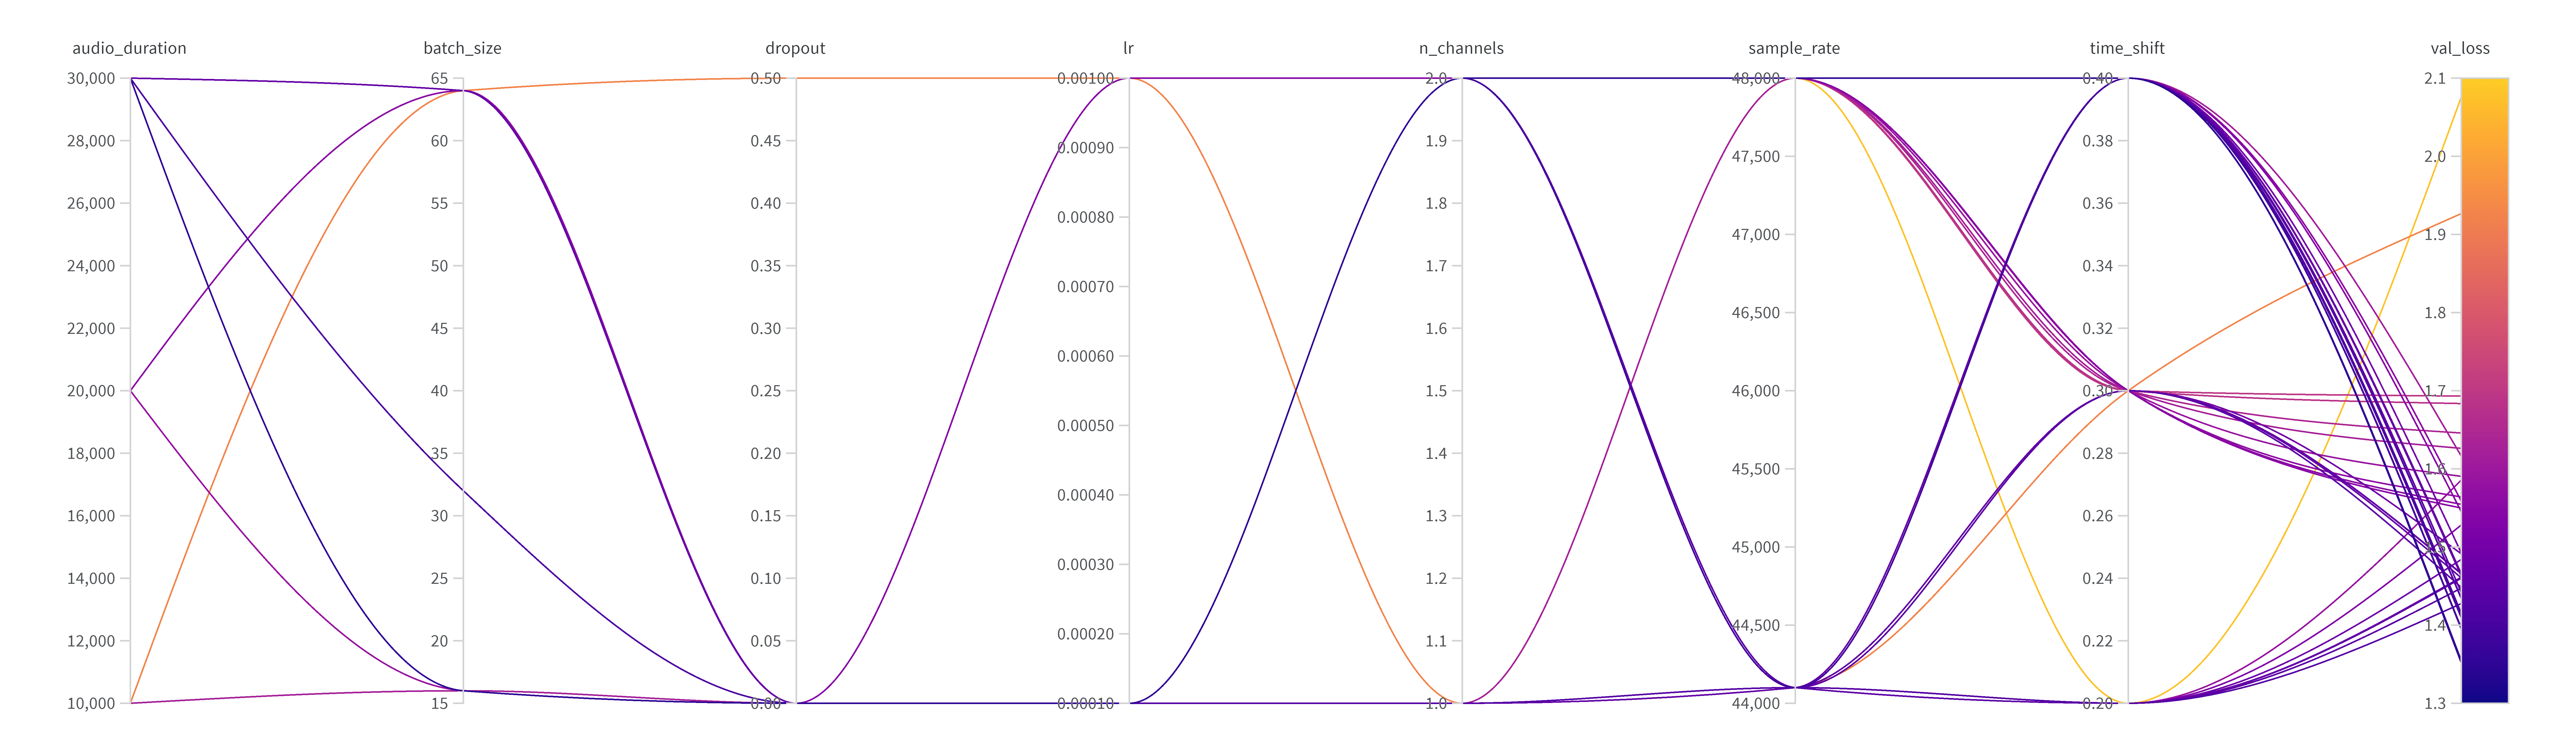
\includegraphics[width=\textwidth]{rsc/sweeps.png}
    \caption{Coût d'entraînement du modèle en fonction des combinaisons de paramètres testées. Chaque combinaison est représentée par une courbe.}
    \label{fig:hyperparameters}
\end{figure}

Les courbes se rapprochant du bleu foncé représentent les combinaisons les plus intéressantes. La combinaison des paramètres minimisant le coût d'entraînement est ensuite utilisée pour l'entraînement du modèle final qui peut ensuite être déployé en production. Au moment de l'écriture de ce rapport, le modèle entraîné possède une \textbf{précision globale de 54 \%} sur les données de test et la matrice de confusion obtenue est illustrée par la figure \ref{fig:confusion_matrix}.

\begin{figure}[H]
    \centering
    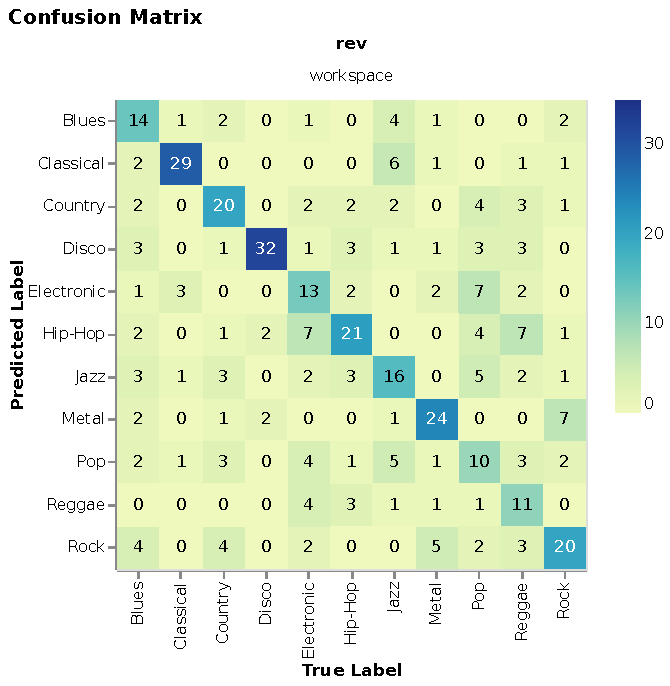
\includegraphics[width=0.5\textwidth]{rsc/confusion_matrix.pdf}
    \caption{Matrice de confusion du modèle entraîné.}
    \label{fig:confusion_matrix}
\end{figure}

La matrice de confusion montre tout de même que la majorité des prédictions se trouvent sur la diagonale. Cependant, le reste des prédictions est très dispersé et il est difficile de dégager une tendance telle que deux classes qui seraient souvent confondues. On peut tout de même noter que la majorité des morceaux classiques et disco sont reconnus correctement avec un recall respectif de 89\% et 83\%. En revanche, les morceaux de pop et de reggae sont les moins bien reconnus avec un recall respectif de 28\% et 31\%. 

Cette dispersion des résultats montre qu'il est difficile pour le modèle de différencier les morceaux par leur genre musical et qu'il n'est pas capable d'apprendre des caractéristiques assez discriminantes pour effectuer cette tâche. Cela peut être en partie dû au fait que les morceaux de musique n'ont pas nécessairement qu'un seul genre musical qui leur est associé. En effet, il est courant de trouver des morceaux de musique qui sont un mélange de plusieurs genres musicaux. La sortie du réseau indiquant, d'une certaine manière, la probabilité d'appartenance à chaque genre musical, il serait possible de donner à chaque genre un certain poids lors de la génération de l'image. Par faute de temps, tout comme la considération d'autres modèles, cette piste n'a pas été explorée dans ce projet.

\subsection{Fonctionnement du service}

Lors de son déploiement, le service télécharge la dernière version du modèle qui est versionnée par DVC et stockée dans notre serveur de stockage MinIO, puis le charge dans son code. À chaque requête effectuée au service, le fichier audio est pré-traité pour générer le spectrogramme correspondant qui est donné en entrée du modèle afin d'obtenir le résultat de la classification et l'envoyer comme réponse.

À noter que le modèle doit recevoir en entrée une donnée audio d'une certaine durée (30 secondes) alors que les fichiers fichiers audio reçus en entrée du service sont souvent plus longs. Si c'est le cas, le service tronque l'audio au milieu de manière à analyser ses parties les plus importantes. En effet, le début d'une musique n'est pas toujours très représentatif de son genre musical global.

\section{Sentiment Analysis}
Afin de ne pas passer directement la transcription de la voix au service de génération d'image, un service d'analyse de sentiment est ajouté. Ce dernier retourne plusieurs informations:

\begin{itemize}
    \item \textbf{Langage:} la langue détectée dans le texte.
    \item{\textbf{Sentiment:} la liste des probabilités par sentiment de la liste suivante:
        \begin{itemize}
            \item Joie
            \item Tristesse
            \item Colère
            \item Surprise
            \item Dégoût
            \item Peur
        \end{itemize}
    }
    \item \textbf{Top words:} les 10 mots les plus "importants" dans le texte.
\end{itemize}

\subsection{Analyse de sentiments}
Pour l'analyse de sentiments, la librairie Pysentimiento \cite{Pysentimiento}, dédiée à cette tâche, est utilisée. À l'aide de cette dernière, il est possible de ressortir le sentiment (positif, neutre, négatif) et les émotions d'un texte. C'est cette deuxième fonctionnalité qui est utilisée. Le modèle de NLP utilise des transformers pré-entraînés (BETO et BERTweet) provenant de HuggingFace.

Avant cela, des essais en utilisant GPT3 ont été effectués afin de générer une phrases à l'aide du texte, mais cette idée a été écartée afin d'éviter des coûts et que le micro-service soit trop orienté vers les pochettes d'album.

\subsection{Mots-clé}
Pour la partie "Top words" une combinaison de plusieurs fonctions permettent de récupérer les 10 mots-clé les plus importants. On utilise la méthode de TF-IDF afin d'analyser l'importance de chaque terme dans le texte. Avant cela, quelques pré-traitements permettent, à l'aide de NLTK et Spacy, de tokenizer les mots et de supprimer les stop words et la ponctuation qui risquent de fausser le calcul.

Enfin, on utilise les mots restants dans le calcul du TF-IDF et on attribue pour chacun des mots un score. Ainsi, il est possible de les classer selon ce dernier et d'avoir les mots-clés les plus importants.

\section{Text Summarizer}
En fin de projet, pour essayer d'avoir des résultats différents (meilleurs?), un dernier micro-service est implémenté et permet de résumer le texte en quelques phrases afin d'éviter de perdre trop d'informations.

Les transformers de HuggingFace contiennent des modèles pré-entraînés qui permettent d'éviter de perdre trop de temps de développement. Après avoir essayé plusieurs modèles différents, "bart-large-cnn-samsum" est celui qui est choisi. Comme paramètre, on limite la sortie à une longueur de 100 mots.

Au final, ce service n'est pas intégré à notre pipeline, par manque de temps pour tester les résultats.

\clearpage

\section{Art Generator}
Le service \textit{Art Generator} est l'ultime étape de la pipeline. En effet, ce dernier est responsable de générer 3 covers d'album différentes à partir des données fournies par les autres micro-services. 
Il prend, en entrée, les thèmes principaux et le sentiment des paroles qui sont issus du service \textit{Sentiment Analysis}, 
ainsi que le genre musical issu du service \textit{Genre Detection}. 

Il existe de nombreux modèles de génération d'images à partir de texte mais le modèle qui est choisi est Stable Diffusion \cite{stable-diffusion}. En effet, il s'agit de l'un des meilleurs dans le domaine de génération d'images à partir de texte. Il a surtout l'avantage de pouvoir être utilisé en local contrairement à d'autres modèles comme DALL-E \cite{dall-e} ou Midjourney \cite{midjourney}, pour lesquels il faut passer par une API payante.

La création d'une pipeline de génération d'images Stable Diffusion est relativement simple grâce à la librairie Diffusers \cite{diffusers} de HuggingFace. Cette dernière permet d'en créer en quelques lignes de code. Il suffit de spécifier le modèle à utiliser ainsi que le prompt, qui est le texte à partir duquel l'image sera générée. La communauté autour de la librairie Diffusers est très active et il existe de nombreux modèles
fine-tunés qui sont compatibles avec cette dernière, ainsi que beaucoup d'autres téléchargeables librement qui sont intégrables dans la pipeline Stable Diffusion.

\subsection{Prompt engineering}
Le prompt est le texte à partir duquel l'image sera générée. Il est donc important de bien le choisir afin d'obtenir des résultats
satisfaisants. De nombreux essais ont été effectués afin de trouver le meilleur prompt, qui est le suivant:

"An album cover in style of \textit{\{music\_style\}} with a sentiment of \textit{\{predominant\_sentiment\}} without any text and illustrating the following themes: \textit{\{main\_themes\}}"

Les paramètres de ce prompt sont les suivants:

\begin{itemize}
    \item \textbf{music\_style:} le genre musical de la chanson qui est issu du service \textit{Genre Detection}.
    \item \textbf{predominant\_sentiment:} le sentiment principal ressenti dans les paroles qui est issu du service \textit{Sentiment Analysis}.
    \item \textbf{main\_themes:} les principaux mots-clés de la chanson qui sont également issus du service \textit{Sentiment Analysis}.
\end{itemize}

\subsubsection*{Negative prompts}

La librairie \textit{Diffusers} permet de générer des images en spécifiant un prompt négatif. 
Il s'agit d'une description de ce que l'image ne doit pas contenir. De nombreux essais ont également été effectués afin de trouver le meilleur prompt négatif qui est le suivant:

"font, typo, signature, text, watermark, cropped, disfigured, duplicate, error, jpeg artifacts, low quality, lowres, mutated hands, out of frame, worst quality"

Il s'agit d'une liste de mots-clés qui est censée permettre d'éviter que l'image générée ne contienne des éléments indésirables, notamment des éléments de texte qui sont dénués de sens car Stable Diffusion n'a pas la capacité de générer des images avec du texte.

Malgré cela, il arrive que certaines images générées contiennent des éléments de texte et cela est dû au fait que la majorité des pochettes d'albums en contiennent. Le modèle a donc tendance à générer des images avec du texte malgré le prompt négatif.

\subsubsection*{Prompt embedding}
Le prompt embedding est une technique qui permet de donner plus de poids à certains mots du prompt.
Cela permet de guider le modèle vers une certaine direction. Par exemple, si l'on souhaite que le modèle génère une image avec un sentiment positif, on peut donner plus de poids au mot "happy".

Pour ce faire, la librairie Compel \cite{compel} est utilisée. Elle permet de donner plus ou moins de poids à certains mots du prompt très facilement
en ajoutant des "++" ou des "--" à la fin de ces derniers. Par exemple, si l'on souhaite donner plus de poids au mot "happy", il suffit d'écrire "happy++" dans le prompt.

\subsection{Modèles utilisés}
Afin de générer des images dans plusieurs styles, trois modèles différents sont utilisés. Cela permet d'obtenir des images plus variées, d'éviter qu'elles ne se ressemblent trop et donc d'avoir des résultats plus intéressants.

Le premier modèle utilisé est \textit{stabilityai/stable-diffusion-2-base} \cite{stabilityai/stable-diffusion-2-base}. 
Il s'agit du modèle de base de Stable Diffusion dans sa version 2. Il est disponible sur HuggingFace et est donc très facilement intégrable dans la pipeline.

Le second modèle utilisé est \textit{prompthero/openjourney} \cite{prompthero/openjourney}. 
Il s'agit d'un modèle qui a été finetuné sur le dataset du très célèbre Midjourney \cite{midjourney} afin d'en imiter le style.
Ce modèle est également disponible directement sur HuggingFace.

Finalement, le dernier modèle et celui qui est le plus difficile à intégrer dans la pipeline est
\textit{Album Cover Art} qui est disponible sur le site CivitAI \cite{civit-ai} qui regroupe de nombreux modèles fine-tunés.
Ce modèle est réglé sur un dataset de pochettes d'albums et permet donc de générer des images ressemblant réellement à des pochettes d'albums. Mais, une fois encore, l'auteur explique que le principal problème de ce modèle est le manque de contrôle sur le texte généré sur les images. Ce modèle n'est pas directement intégrable dans la pipeline Stable Diffusion car il est uniquement disponible en tant que modèle PyTorch qui est un fichier \textit{.ckpt} de plusieurs GB. Il a donc été nécessaire de le convertir en une pipeline HuggingFace afin qu'il puisse être utilisé de la même manière que les autres modèles.

\subsection{Exemple de génération d'images}
La figure \ref{fig:generation_result} Résultat obtenu avec la chanson "Fear of the dark" de Iron Maiden.

\begin{figure}[H]
    \centering
    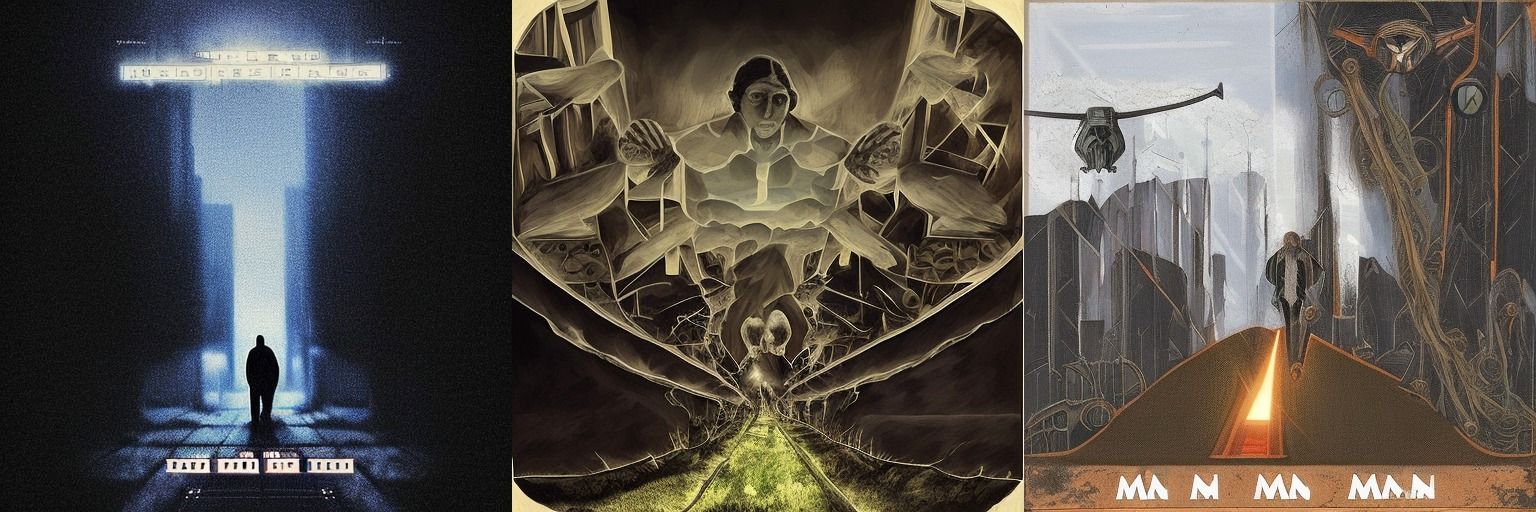
\includegraphics[width=1\textwidth]{rsc/results_art_generation.jpeg}
    \caption[Exemple d'images générées par chaque modèle]{Exemple d'images générées par chaque modèle (de gauche à droite : \textit{Album Cover Art}, \textit{prompthero/openjourney}, \textit{stabilityai/stable-diffusion-2-base})}
    \label{fig:generation_result}
\end{figure}

\subsubsection*{Prompt utilisé}

Ce prompt a été généré par le service en se basant sur les différentes informations données par les autres services de la pipeline.

"An album cover in style of Metal with a fear sentiment without any text and illustrating the following themes: man++++++, walk++++, dark++, night, park, fear, little, anxious"

\subsubsection*{Paramètres de générations}
Les paramètres de générations sont les mêmes que ceux utilisés par le service.
\begin{itemize}
    \item \textbf{guidance\_scale}: \textbf{5} 
    
    Ce paramètre permet de contrôler l'importance accordée au prompt lors de la génération d'une image. En d'autres termes, il représente l'influence du signal de conditionnement sur le processus de génération d'image. 
    \item \textbf{nb\_steps}: \textbf{50}

    Ce paramètre indique le nombre d'itérations que le modèle effectue pour générer l'image. Plus il est grand plus l'image sera "détaillée" mais plus le temps de génération sera lent. Il est choisi de générer les images en 50 itérations car c'est un bon compromis entre performance et qualité.
\end{itemize}





